\usetikzlibrary{calc}

% Control Parameters
\newcommand\moonangle{24}
\newcommand\primeaxisext{0.9}
\newcommand\moonext{0.7}
\newcommand\earthext{0.1}
\newcommand\earthlineext{0.3}
\newcommand\projext{0.4}

% The Actual Drawing 
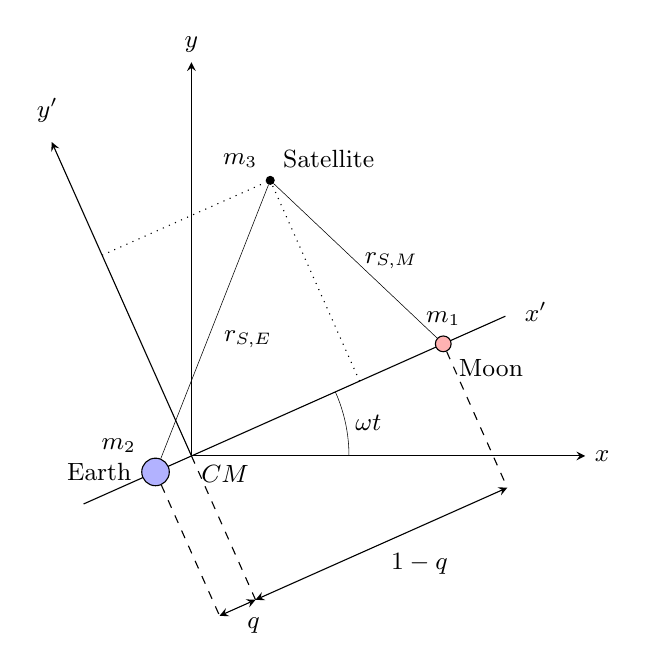
\begin{tikzpicture}[>=stealth, scale=5, z={(-0.5cm,-0.4cm)}]
	\tikzstyle{every node}=[font=\small]
	
	%origo
	\coordinate[label=below right:$CM$] (O) at (0,0,0) {};
	
	%xy axes
	\draw[->] (O) -- +(1,0) node [right] {$x$};
	\draw[->] (O) -- +(0,1) node [above] {$y$};
	
	%y'
	\node (yprime) at (90+\moonangle:\primeaxisext) {};
	\draw[->] (O) -- (yprime) node [above] {$y^{\prime}$};
	
	%x' 
	\node (xprime) at (\moonangle:\primeaxisext) {};
	\draw (O) -- (xprime) node [right]{$x^{\prime}$};
	
	%arc
	\draw[very thin] (O) +(0.4,0,0) arc (0:\moonangle:0.4);
	\draw (O) +(\moonangle/2:0.4) node [right] {$\omega t$};
	
	% Earth, Satellite, Moon
	\draw (O) -- (\moonangle+180:\earthlineext);
	
	\node[label=above right:Satellite, label=above left:$m_3$, circle, draw, fill=black, inner sep=0pt, minimum size=0.1cm] (S) at (0.2,0.7) {};
	\node[label=left:Earth, label=above left:$m_2$, circle, draw, fill=blue!30, inner sep=0pt, minimum size=0.35cm] (E) at (\moonangle+180:\earthext) {};
	\node[label=below right:Moon, label=above:$m_1$, circle, draw, fill=red!30, inner sep=0pt, minimum size=0.2cm] (M) at (\moonangle:\moonext) {};
	
	%projections
	\draw[very thin] (E) -- (S) node[midway] [below right]{$r_{S,E}$} -- (M) node[midway] [right] {$r_{S,M}$};
	\draw[dotted] ($(O)!(S)!(yprime)$) -- (S); % projection from calc library
	\draw[dotted] ($(O)!(S)!(xprime)$) -- (S); % projection from calc library
	
	\coordinate (p1) at (-90+\moonangle:\projext);
	\coordinate (p2) at ($ (p1) + (E) $);
	\coordinate (p3) at ($ (p1) + (\moonangle:\moonext) $);
	
	\draw[<->] (p1) -- (p2) node[midway, below right]{$q$};
	\draw[<->] (p1) -- (p3) node[midway, below right]{$1-q$};
	\draw[dashed] (O) -- (p1) (E) -- (p2) (M) -- (p3);
\end{tikzpicture}


